\begin{solution}{Question 4}\label{ques:4}
    \begin{question}
    Let Commit be a single-bit commitment scheme. Show that if Commit satisfies the collapse-binding property, then it also satisfies prof-binding.
    \end{question}
    \tcblower{}
    \begin{proof}
    To prove that collapse binding implies prof binding, we will show a reduction where if the adversary breaks prof binding with some non negligible probability $\epsilon$, the reduction breaks collapse-binding with some non negligibile probability $\mathcal{O}(\epsilon)$. Let the games for collapse-binding and sum-binding be defined as follows:\\
    \begin{figure}[H]
      \begin{subfigure}[b]{0.5\textwidth}
        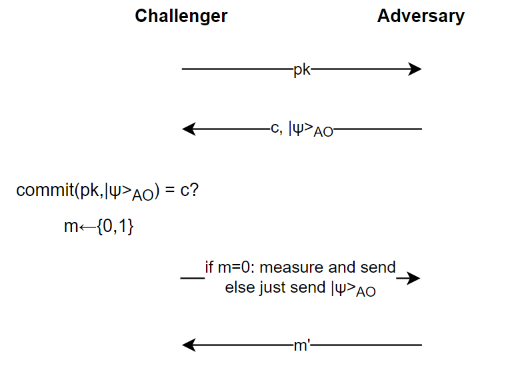
\includegraphics[width=\textwidth]{images/collapse.png}
        \caption{Collapse-binding}
        \label{fig:cb}
      \end{subfigure}
      \hfill
      \begin{subfigure}[b]{0.48\textwidth}
        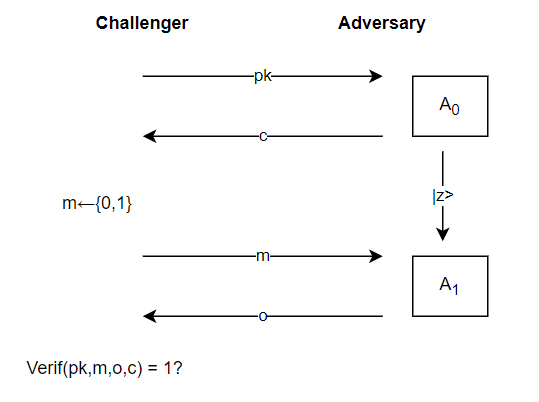
\includegraphics[width=\textwidth]{images/prof.png}
        \caption{Prof binding}
        \label{fig:prof}
      \end{subfigure}
      \caption{Games for the two commitment schemes}
    \end{figure}

    % \begin{definition}Collapse-binding: (equivalent to the definition provided in class) \\
    % For algorithms $(A, B)$, consider the following games:
    % \begin{equation}
    %     \begin{split}
    %     \text{Game}_1 &: k \leftarrow \bfP, (S, M, U, c) \leftarrow A(k), m \leftarrow \calM(M), b \leftarrow B(S, M, U)\\
    %     \text{Game}_2 : k \leftarrow \bfP, (S, M, U, c) \leftarrow A(k), b \leftarrow B(S, M, U)
    %     \end{split}
    % \end{equation}

    % Here $S, M, U$ are quantum registers and $c,m,u$ are commitment, message and the opening respectively. $verify(k, c, m, u)$ checks if u is a valid opening for commitment c of m.  $\calM(M)$ is measurement of $M$ in the computational basis.\\

    % Now, an adversary (A, B) is collapse binding-valid for verify $iff$ for all k, $\prob{verify(k, c, m, u) = 1} =1$ when we run $(S, M, U, c) \leftarrow A(k)$ and measure $M$ in the computational basis as $m$, and $U$ in the computational basis as $u$.\\
    
    % A commitment scheme is collapse-binding iff for any qpt adversary $(A, B)$ that is collapse binding-valid for verify, $\prob{b = 1 : Game_1} - \prob{b = 1 : Game_2}$ is negligible.
    % \end{definition}
    % \begin{definition}Prof-binding: For any adversary $(C_0, C_1)$ and $m\in \{0,1\}$, 
    % \begin{equation}
    %     p_m(C_0, C_1) := \prob{\texttt{verify}(k, c, m, u) = 1 : k \leftarrow \bfP,(S, c) \leftarrow C_0(k), u \leftarrow C_1(S, m)}
    % \end{equation}
    % Where $S$ is a quantum register, and c is a classical value. $C_0$ generates the commitment and $C_1$ gets an opening u for m. The advantage of adversary is defined as: $p_0+p_1-1$
    % \end{definition}
    

    % Since the adversary is a quantum algorithm, a rewinding proof does not work, hence we will run the queries in superposition. 
    
    \end{proof}
\end{solution}
 